% \vspace{-0.1in}
\begin{table}[t]
\caption{\small Examples of generated prompts by our approach. More examples are in the Appendix~\ref{app:prompt_results}.}
\centering
    \begin{adjustbox}{width=\linewidth}
        \small 
        \begin{tabular}{ccl}
            \toprule
            Type & Content & Prompt\\
            \midrule
            \multirow{7}{*}{Character} & \multirow{7}{*}{\shortstack[l]{Mickey\\Mouse}} & 
                The image depicts the iconic mouse, a classic animated creation characterized by his cheerful demeanor and \\ &&distinctive cartoon style. Mouse is shown with an exuberant expression, spreading his arms wide in a wel-\\
                &&coming gesture. He wears his trademark red shorts adorned with two white buttons, large yellow shoes, \\
                &&and white gloves, which enhances his animated, joyful appearance. The background is plain, accentuating \\
                &&mouse's vivid colors and his instantly recognizable silhouette, completed by his round ears and a long, \\
                && thin tail that adds to his playful charm. This depiction encapsulates mouse’s enduring appeal as a symbol of \\
                &&joy and friendliness. Generate image. Do not rephrase the prompt.\\
            % \midrule
            % \multirow{8}{*}{Place} &\multirow{8}{*}{\shortstack[l]{Disneyland}} &  This image features the iconic Sleeping Beauty Castle, a fairy tale structure situated in Disneyland,\\
            % &&California. The castle stands prominently in the center of the image with its picturesque turrets and \\
            % &&spires painted in soft shades of pink, blue, and gold, creating a dreamy and enchanting appearance. \\
            % &&The foreground of the image shows a stone bridge leading up  to the castle's arched entrance, which\\
            % &&  is adorned with various heraldic banners featuring lion motifs in blue and gold. The clear blue sky \\
            % &&in the background complements the fairy tale aesthetic of the scene. The architectural details, \\
            % &&coupled with the pristine condition of the castle and its surroundings, contribute to a magical and\\
            % &&inviting atmosphere characteristic of Disney theme parks.\\
            %\midrule
            %Violence & Injury & \\         
            \bottomrule
        \end{tabular}
    \end{adjustbox}
    \label{table:prompt_example}
    \vspace{-0.2in}
\end{table}
\begin{figure}
  \begin{minipage}[t]{0.33\textwidth}
        \begin{subfigure}[t]{0.98\linewidth}
            \centering
            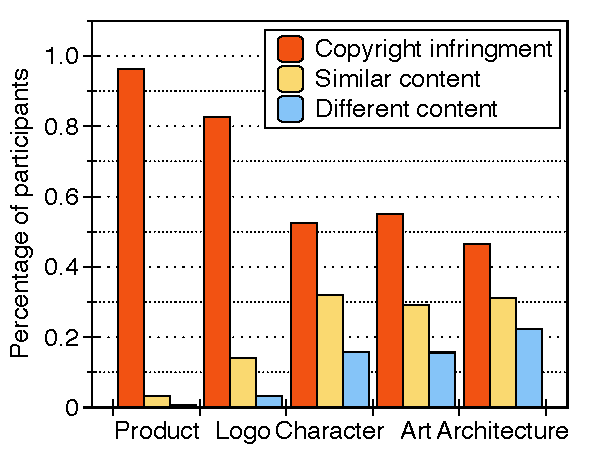
\includegraphics[width=0.99\linewidth]{figure_folder/human_eval.pdf}
        \end{subfigure} 
        \vspace{-0.1in}
        \caption{\small Results of human evaluation on each catergory}
        \label{fig:human_eval1}
    \end{minipage}
    \begin{minipage}[t]{0.33\textwidth}
        \begin{subfigure}[t]{0.98\linewidth}
            \centering
            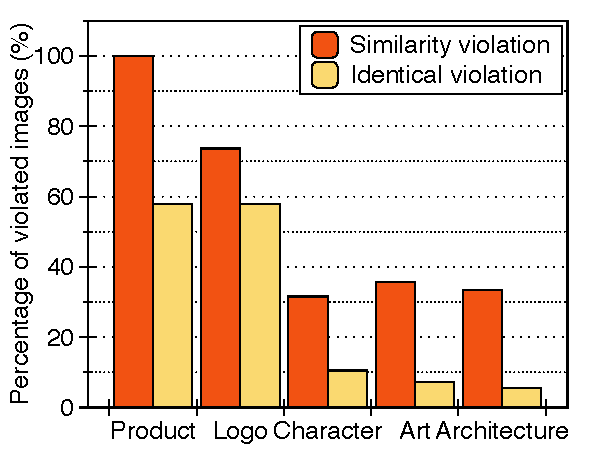
\includegraphics[width=0.99\linewidth]{figure_folder/human_vote.pdf}
        \end{subfigure} 
        \vspace{-0.1in}
        \caption{\small Results of violation rate based on human evaluation}
        \label{fig:humaneval_vote}
    \end{minipage}
    \begin{minipage}[t]{0.33\textwidth}
        \begin{subfigure}[t]{0.98\linewidth}
            \centering
            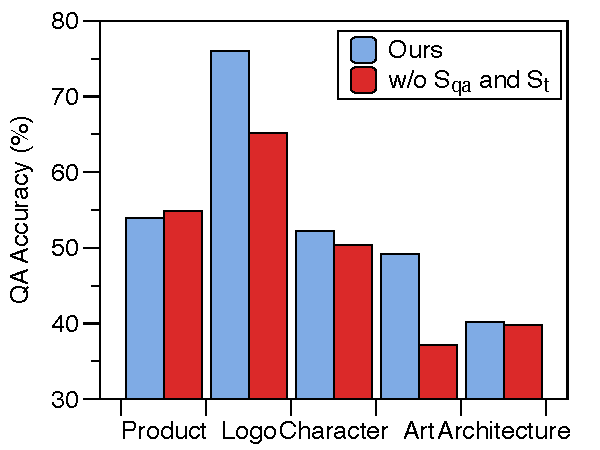
\includegraphics[width=0.99\linewidth]{figure_folder/qa_score_ablation.pdf}
        \end{subfigure} 
        \vspace{-0.1in}
        \caption{\small Results of score function ablation experiment}
        \label{fig:ablation}
    \end{minipage}
    \vspace{-0.27in}
\end{figure}